%%%%%%%%%%%%%%%%%%%%%%%%%%%%%%%%%%%%%%%%%
% Beamer Presentation
% LaTeX Template
% Version 2.0 (March 8, 2022)
%
% This template originates from:
% https://www.LaTeXTemplates.com
%
% Author:
% Vel (vel@latextemplates.com)
%
% License:
% CC BY-NC-SA 4.0 (https://creativecommons.org/licenses/by-nc-sa/4.0/)
%
%%%%%%%%%%%%%%%%%%%%%%%%%%%%%%%%%%%%%%%%%

%----------------------------------------------------------------------------------------
%	PACKAGES AND OTHER DOCUMENT CONFIGURATIONS
%----------------------------------------------------------------------------------------

\documentclass[
	10pt, % Set the default font size, options include: 8pt, 9pt, 10pt, 11pt, 12pt, 14pt, 17pt, 20pt
	%t, % Uncomment to vertically align all slide content to the top of the slide, rather than the default centered
	%aspectratio=169, % Uncomment to set the aspect ratio to a 16:9 ratio which matches the aspect ratio of 1080p and 4K screens and projectors
]{beamer}

\graphicspath{{figures/}{./}} % Specifies where to look for included images (trailing slash required)


\usepackage{booktabs} % Allows the use of \toprule, \midrule and \bottomrule for better rules in tables
\usepackage{multimedia}
\usepackage{hyperref}
\usepackage{outlines}
\usepackage{float}
% \usepackage{caption}
\usepackage{subcaption}
%----------------------------------------------------------------------------------------
%	SELECT LAYOUT THEME
%----------------------------------------------------------------------------------------

% Beamer comes with a number of default layout themes which change the colors and layouts of slides. Below is a list of all themes available, uncomment each in turn to see what they look like.

%\usetheme{default}
%\usetheme{AnnArbor}
%\usetheme{Antibes}
%\usetheme{Bergen}
%\usetheme{Berkeley}
%\usetheme{Berlin}
%\usetheme{Boadilla}
%\usetheme{CambridgeUS}
%\usetheme{Copenhagen}
%\usetheme{Darmstadt}
%\usetheme{Dresden}
%\usetheme{Frankfurt}
%\usetheme{Goettingen}
%\usetheme{Hannover}
%\usetheme{Ilmenau}
%\usetheme{JuanLesPins}
%\usetheme{Luebeck}
\usetheme{Madrid}
%\usetheme{Malmoe}
%\usetheme{Marburg}
%\usetheme{Montpellier}
%\usetheme{PaloAlto}
%\usetheme{Pittsburgh}
%\usetheme{Rochester}
%\usetheme{Singapore}
%\usetheme{Szeged}
%\usetheme{Warsaw}

%----------------------------------------------------------------------------------------
%	SELECT COLOR THEME
%----------------------------------------------------------------------------------------

% Beamer comes with a number of color themes that can be applied to any layout theme to change its colors. Uncomment each of these in turn to see how they change the colors of your selected layout theme.

% \usecolortheme{albatross}
%\usecolortheme{beaver}
%\usecolortheme{beetle}
%\usecolortheme{crane}
%\usecolortheme{dolphin}
%\usecolortheme{dove}
%\usecolortheme{fly}
%\usecolortheme{lily}
%\usecolortheme{monarca}
%\usecolortheme{seagull}
%\usecolortheme{seahorse}
\usecolortheme{spruce}
%\usecolortheme{whale}
% \usecolortheme{wolverine}

%----------------------------------------------------------------------------------------
%	SELECT FONT THEME & FONTS
%----------------------------------------------------------------------------------------

% Beamer comes with several font themes to easily change the fonts used in various parts of the presentation. Review the comments beside each one to decide if you would like to use it. Note that additional options can be specified for several of these font themes, consult the beamer documentation for more information.

\usefonttheme{default} % Typeset using the default sans serif font
%\usefonttheme{serif} % Typeset using the default serif font (make sure a sans font isn't being set as the default font if you use this option!)
%\usefonttheme{structurebold} % Typeset important structure text (titles, headlines, footlines, sidebar, etc) in bold
%\usefonttheme{structureitalicserif} % Typeset important structure text (titles, headlines, footlines, sidebar, etc) in italic serif
%\usefonttheme{structuresmallcapsserif} % Typeset important structure text (titles, headlines, footlines, sidebar, etc) in small caps serif

%------------------------------------------------

%\usepackage{mathptmx} % Use the Times font for serif text
\usepackage{palatino} % Use the Palatino font for serif text

%\usepackage{helvet} % Use the Helvetica font for sans serif text
\usepackage[default]{opensans} % Use the Open Sans font for sans serif text
%\usepackage[default]{FiraSans} % Use the Fira Sans font for sans serif text
%\usepackage[default]{lato} % Use the Lato font for sans serif text

%----------------------------------------------------------------------------------------
%	SELECT INNER THEME
%----------------------------------------------------------------------------------------

% Inner themes change the styling of internal slide elements, for example: bullet points, blocks, bibliography entries, title pages, theorems, etc. Uncomment each theme in turn to see what changes it makes to your presentation.

%\useinnertheme{default}
\useinnertheme{circles}
%\useinnertheme{rectangles}
%\useinnertheme{rounded}
%\useinnertheme{inmargin}

%----------------------------------------------------------------------------------------
%	SELECT OUTER THEME
%----------------------------------------------------------------------------------------

% Outer themes change the overall layout of slides, such as: header and footer lines, sidebars and slide titles. Uncomment each theme in turn to see what changes it makes to your presentation.

%\useoutertheme{default}
%\useoutertheme{infolines}
%\useoutertheme{miniframes}
%\useoutertheme{smoothbars}
%\useoutertheme{sidebar}
%\useoutertheme{split}
%\useoutertheme{shadow}
%\useoutertheme{tree}
%\useoutertheme{smoothtree}

%\setbeamertemplate{footline} % Uncomment this line to remove the footer line in all slides
%\setbeamertemplate{footline}[page number] % Uncomment this line to replace the footer line in all slides with a simple slide count

%\setbeamertemplate{navigation symbols}{} % Uncomment this line to remove the navigation symbols from the bottom of all slides

%----------------------------------------------------------------------------------------
%	PRESENTATION INFORMATION
%----------------------------------------------------------------------------------------

\title[PhD interview presentation]{PhD interview presentation} % The short title in the optional parameter appears at the bottom of every slide, the full title in the main parameter is only on the title page

% \subtitle{Optional Subtitle} % Presentation subtitle, remove this command if a subtitle isn't required

\author[Mikkel Metzsch Jensen]{Mikkel Metzsch Jensen} % Presenter name(s), the optional parameter can contain a shortened version to appear on the bottom of every slide, while the main parameter will appear on the title slide

\institute[UiO]{University of Oslo} % Your institution, the optional parameter can be used for the institution shorthand and will appear on the bottom of every slide after author names, while the required parameter is used on the title slide and can include your email address or additional information on separate lines

\date[\today]{Master's thesis midway presentation \\ January 26, 2023} % Presentation date or conference/meeting name, the optional parameter can contain a shortened version to appear on the bottom of every slide, while the required parameter value is output to the title slide

%----------------------------------------------------------------------------------------

\begin{document}

%----------------------------------------------------------------------------------------
%	TITLE SLIDE
%----------------------------------------------------------------------------------------

\begin{frame}
	\titlepage % Output the title slide, automatically created using the text entered in the PRESENTATION INFORMATION block above
\end{frame}

%----------------------------------------------------------------------------------------
%	TABLE OF CONTENTS SLIDE
%----------------------------------------------------------------------------------------

% The table of contents outputs the sections and subsections that appear in your presentation, specified with the standard \section and \subsection commands. You may either display all sections and subsections on one slide with \tableofcontents, or display each section at a time on subsequent slides with \tableofcontents[pausesections]. The latter is useful if you want to step through each section and mention what you will discuss.

% \begin{frame}
% 	\frametitle{Presentation Overview} % Slide title, remove this command for no title
	
% 	\tableofcontents % Output the table of contents (all sections on one slide)
% 	%\tableofcontents[pausesections] % Output the table of contents (break sections up across separate slides)
% \end{frame}

%----------------------------------------------------------------------------------------
%	PRESENTATION BODY SLIDES
%----------------------------------------------------------------------------------------


\section{Introduction}

\begin{frame}
	\frametitle{Academic Background}
	\framesubtitle{Summary and interest?}

	Education
	\begin{itemize}
		\item Bachelor in physcis 
		\item Master in Computational Science: Materials Science 
	\end{itemize}
	Interest
	\begin{itemize}
		\item Computational approach
		\item Design and creation 
		\item Optimization problems
		\item Machine learning 
	\end{itemize}
\end{frame}


\section{Programming experience}


\begin{frame}
	\frametitle{Programming experience}
	\framesubtitle{High level languages}

	{\large Python} 
	\begin{itemize}
		\item Workhorse of all my work.
		\item Object oriented code.
		\item Machine learning through PyTorch and TensorFlow.
	\end{itemize}

	{\large Julia} 
	\begin{itemize}
		\item Alternative to Python 
		\item Finite element analysis using Gridap
		\item Mesh geometris using Gmsh
	\end{itemize}

	\begin{figure}
		\centering
		\begin{subfigure}[b]{0.32\textwidth}
			\centering
			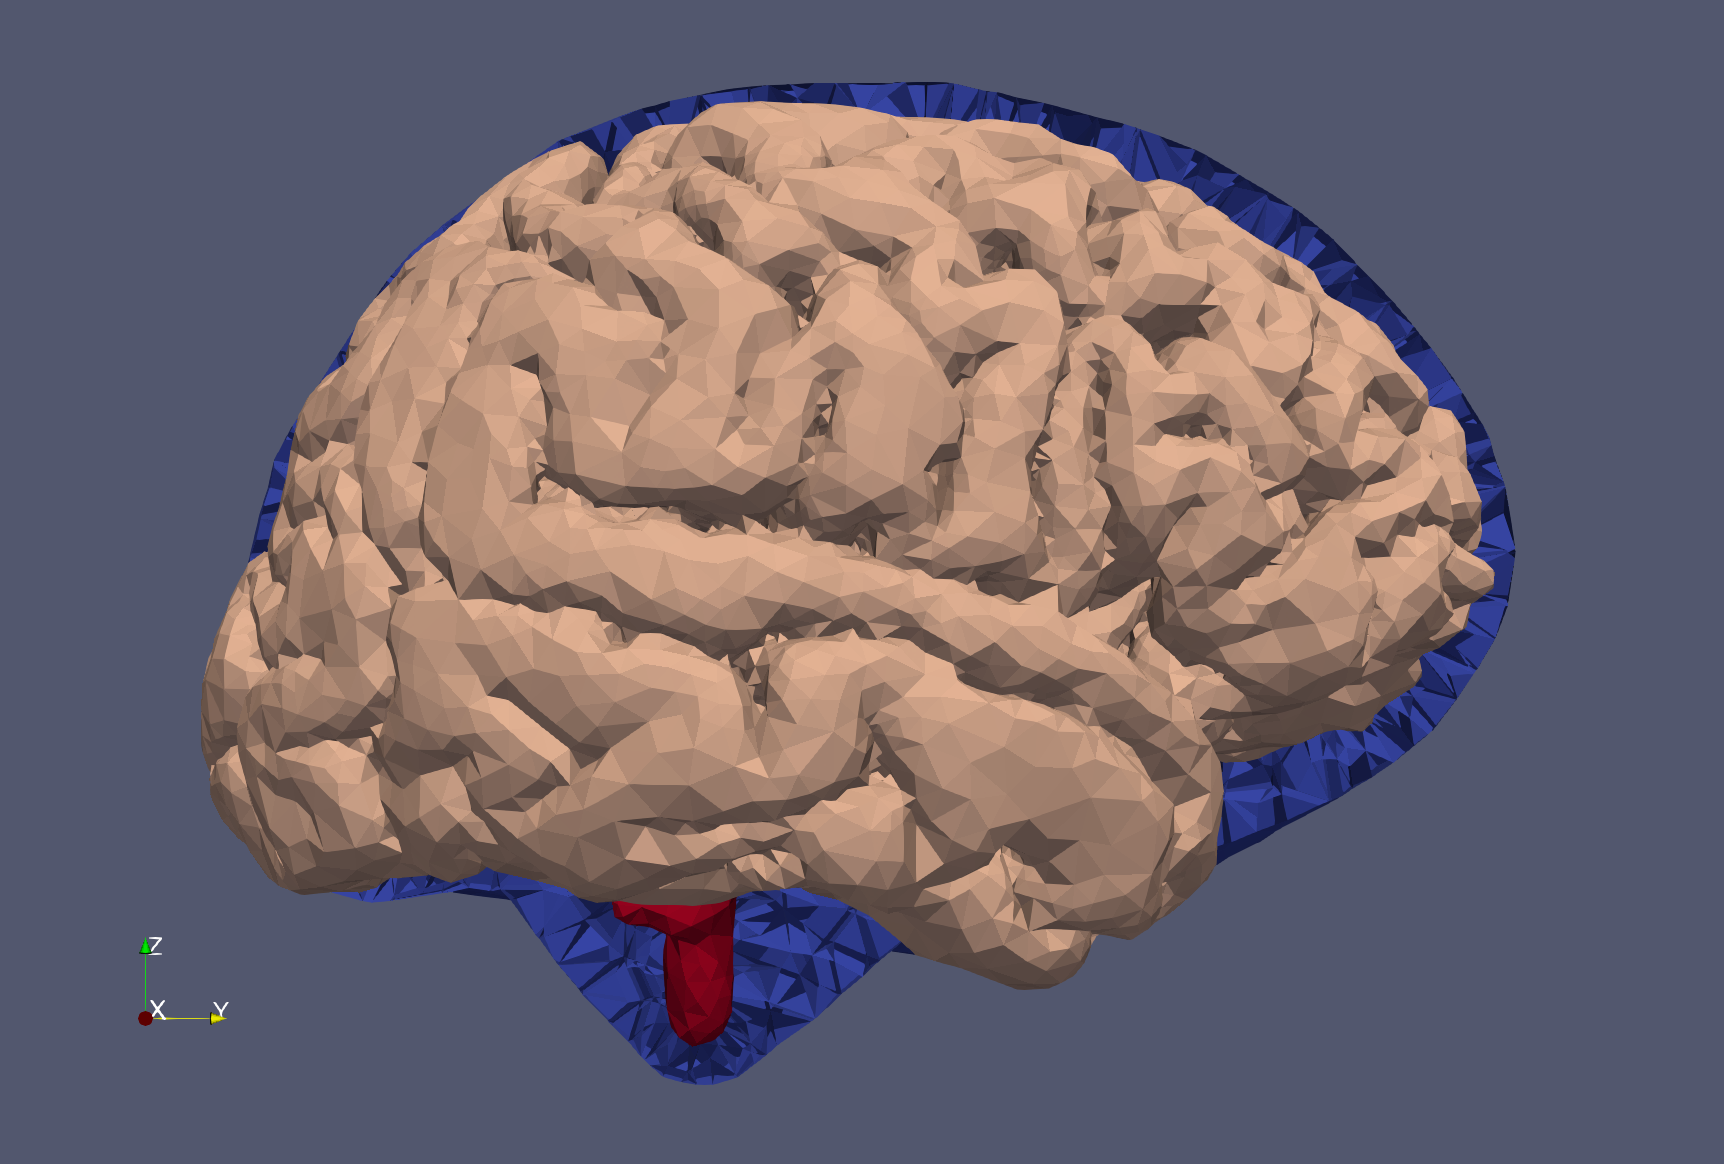
\includegraphics[width=0.70\textwidth]{figures/real_brain_full.png}
			\caption{}
		\end{subfigure}
		\hfill
		\begin{subfigure}[b]{0.32\textwidth}
			\centering
			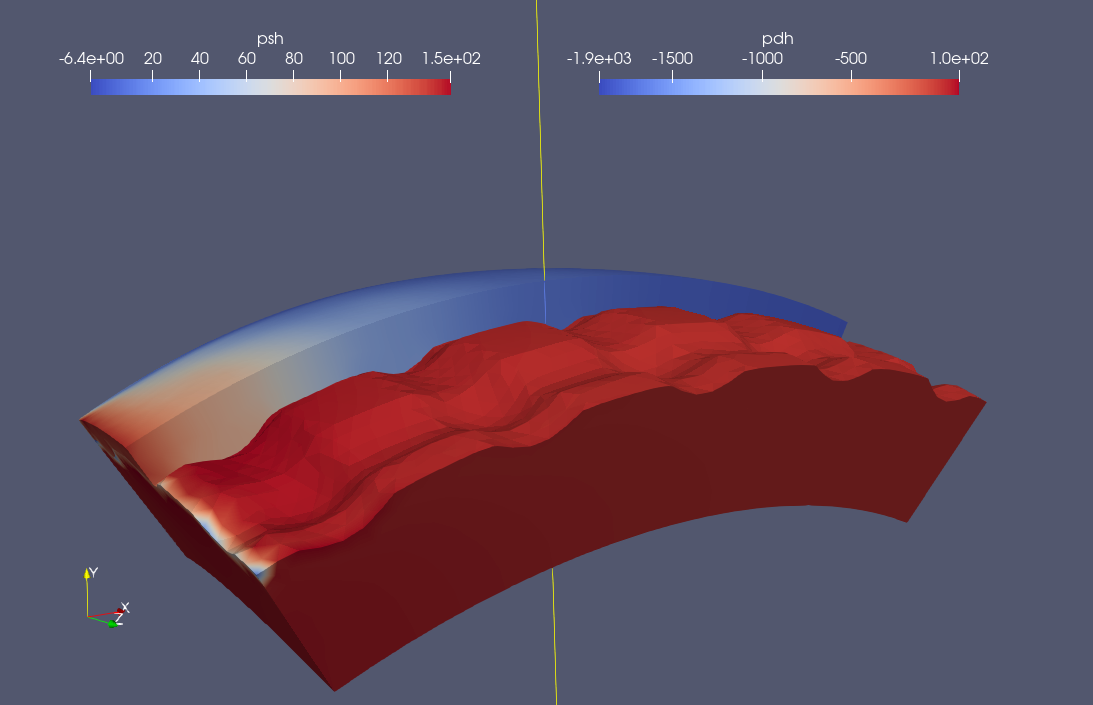
\includegraphics[width=0.70\textwidth]{figures/3D_profile.png}
			\caption{}
		\end{subfigure}
		\hfill
		\begin{subfigure}[b]{0.32\textwidth}
			\centering
			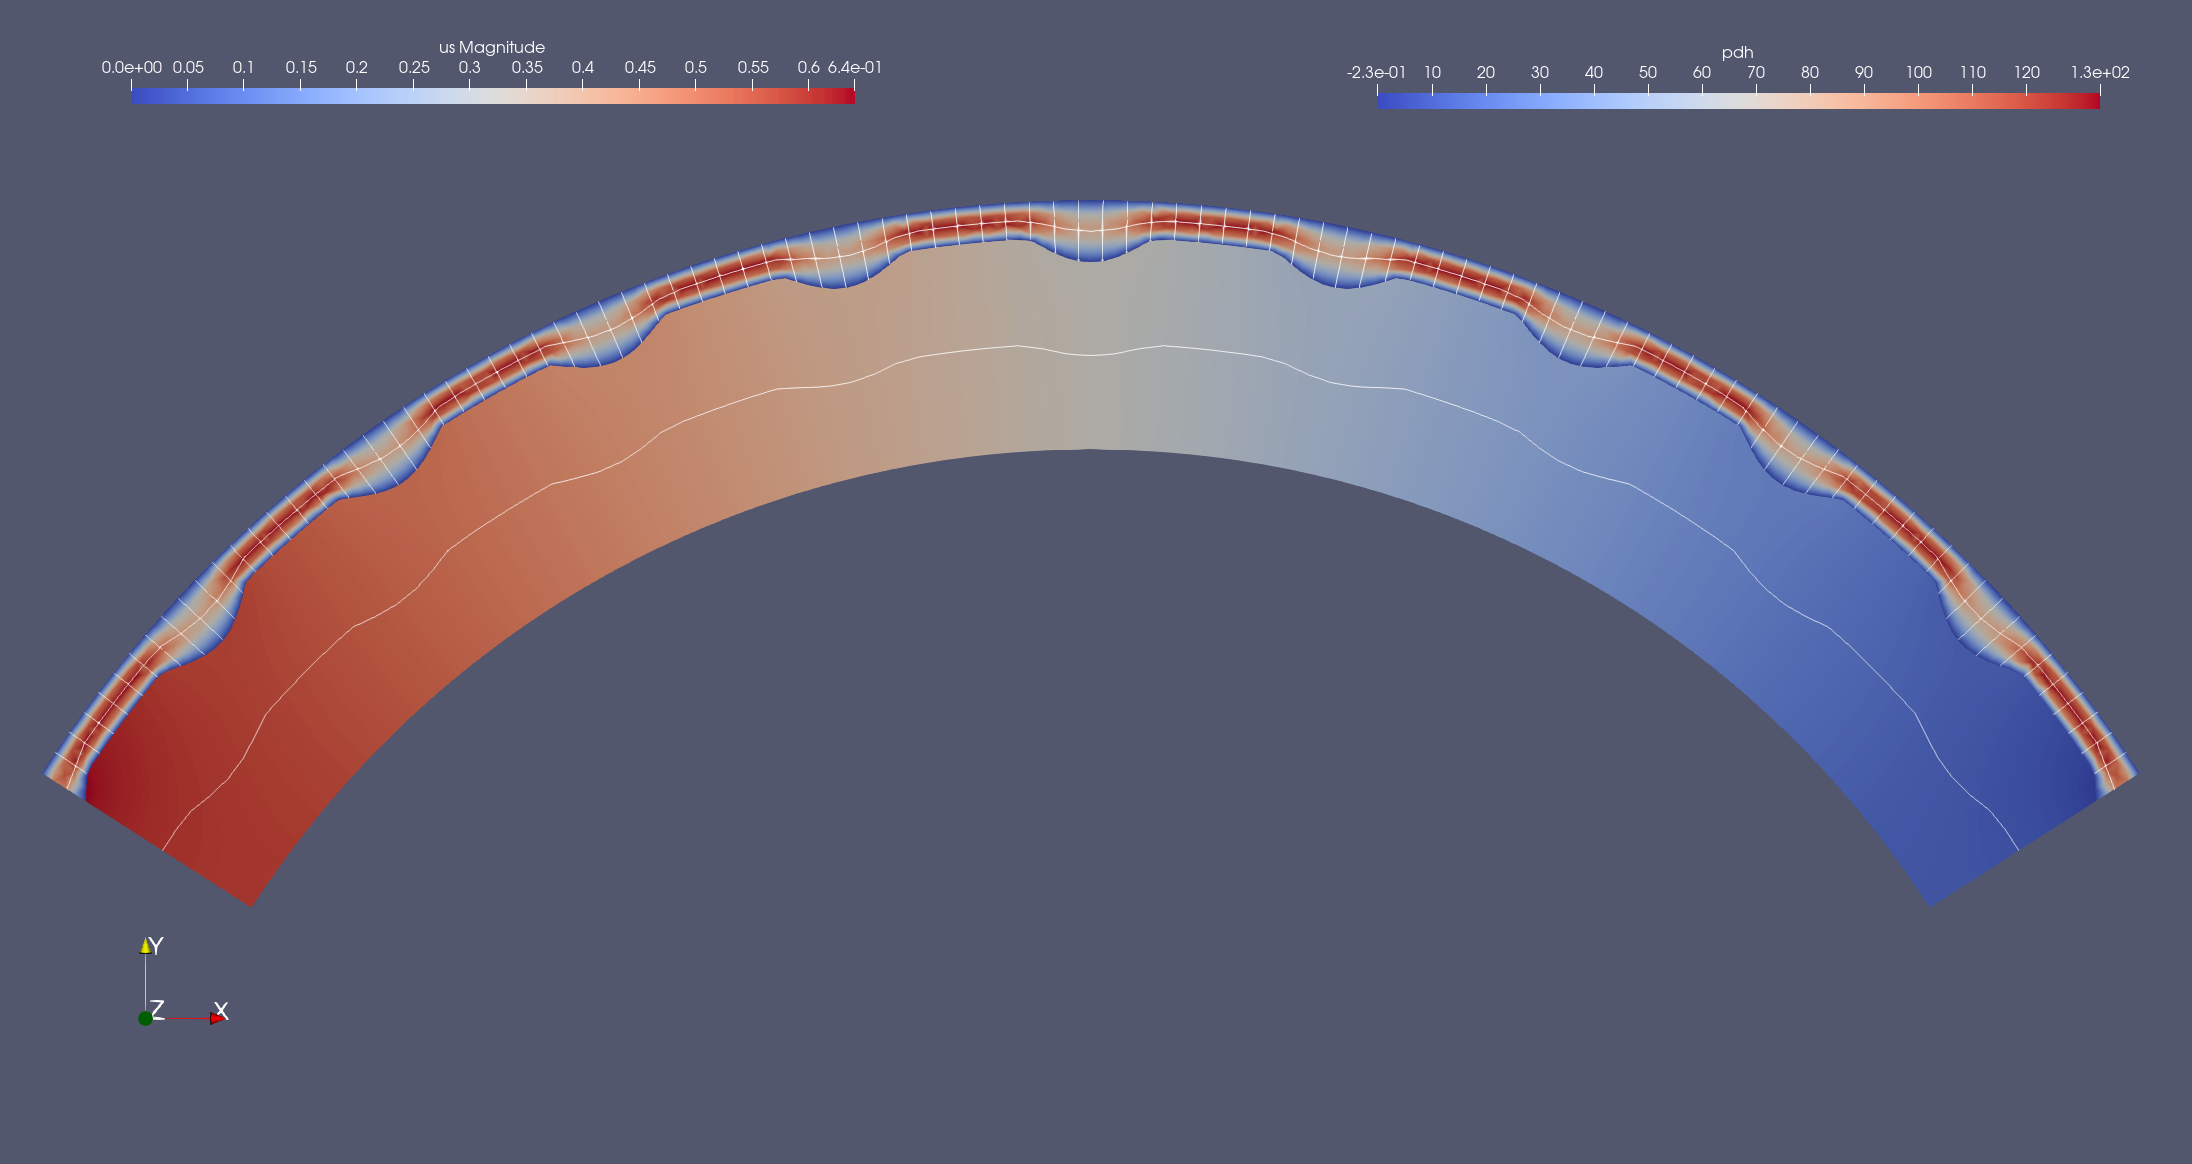
\includegraphics[width=0.85\textwidth]{figures/2D_view.png}
			\caption{}
		\end{subfigure}
		\hfill
		%    \caption{}
	  \end{figure}

\end{frame}


\begin{frame}
	\frametitle{Programming experience}
	\framesubtitle{Lower level languages}

	{\large C++} 
	\begin{itemize}
		\item Object oriented code.
		\item Project work in computational physics.
		\begin{itemize}
			\item [-] Eigenvalue problems and matrix operations.
			\item [-] Ordinary and partial differential equations
			\item [-] Integration 
			\item [-] Simulation of stochastic systems.
		\end{itemize}
		\item Two years teaching assistant.
	\end{itemize}

	% LU decomposition, the Verlet algorithm, Runge-Kutta methods, the Crank-Nicolson method, Gaussian quadrature, Monte Carlo methods, Markov chains, and the Metropolis algorithm.

	{\large C} 
	\begin{itemize}
		\item High performance computing 
		\begin{itemize}
			\item [-] General code optimization.
			\item [-] Data traffic and cache managenemt.
			\item [-] Parallel programming (MPI and OpenMP).
			\item [-] Modern data architecture.
		\end{itemize}
	\end{itemize}

\end{frame}


\begin{frame}
	\frametitle{Programming experience}
	\framesubtitle{Molecular dynamics}

	{\large LAMMPS} \\
	Large-scale Atomic/Molecular Massively Parallel Simulator
	\begin{itemize}
		\item Statistical mechanics and thermodynamics
		\item Structure recognition
		\item Porous systems 
		\item Contact forces
		\item Friction properties
	\end{itemize}


\end{frame}

\begin{frame}
	\frametitle{Programming experience}
	\framesubtitle{Machine learning (ML)}

	{\large Pytorch (/ TensorFlow)} 
	\begin{itemize}
		\item Basic ML concepts: 
		\begin{itemize}
			\item [-] Optimizers
			\item [-] Loss / cost functions
			\item [-] General learning strategies (learning rates, drop out, normalization etc.)
		\end{itemize}
		
		\item Data handling and augmentation.
		\item Fundamental architecture types 
		\begin{itemize}
			\item [-] Feed Forward Networks
			\item [-] CNN
			\item [-] RNN 
			\item [-] GAN
		\end{itemize}
		\item Network performance analysis
		\item Basic basic techniques for AI predictions explainations
		\begin{itemize}
			\item [-] Shapley values 
			\item [-] Gradient linearization methods
		\end{itemize}
	
	\end{itemize}


\end{frame}



% Machine learning
% High performance
% MD Simulations


\section{Master's thesis}


\begin{frame}
	\frametitle{Master's thesis}
	\framesubtitle{Scope}

 
	Tuning frictional properties of graphene sheets using kirigami inspired cuts and inverse design
	\newline
	\newline
	


	\begin{enumerate}
		\setlength\itemsep{2em}
		\item \underline{Sheet kirigami}: Alter graphene sheet using atomic scale cuts. % Buckling in the 3rd dimension
		\item \underline{Forward simulation}: Calculate frictional properties of the sheet using MD simulations.
		\item \underline{Inverse design}: Predict cut patterns based on frictional properties and optimize for desired properties using machine learning.
		\begin{itemize}
			\item Low / high friction coefficient.
			\item Coupling between stretch and friction.
		\end{itemize} 
	\end{enumerate}

\end{frame}



\begin{frame}
	\frametitle{Master's thesis}
	\framesubtitle{Motivation}

	Kirigami: Variation of origami with cuts permitted.

	\begin{figure}
		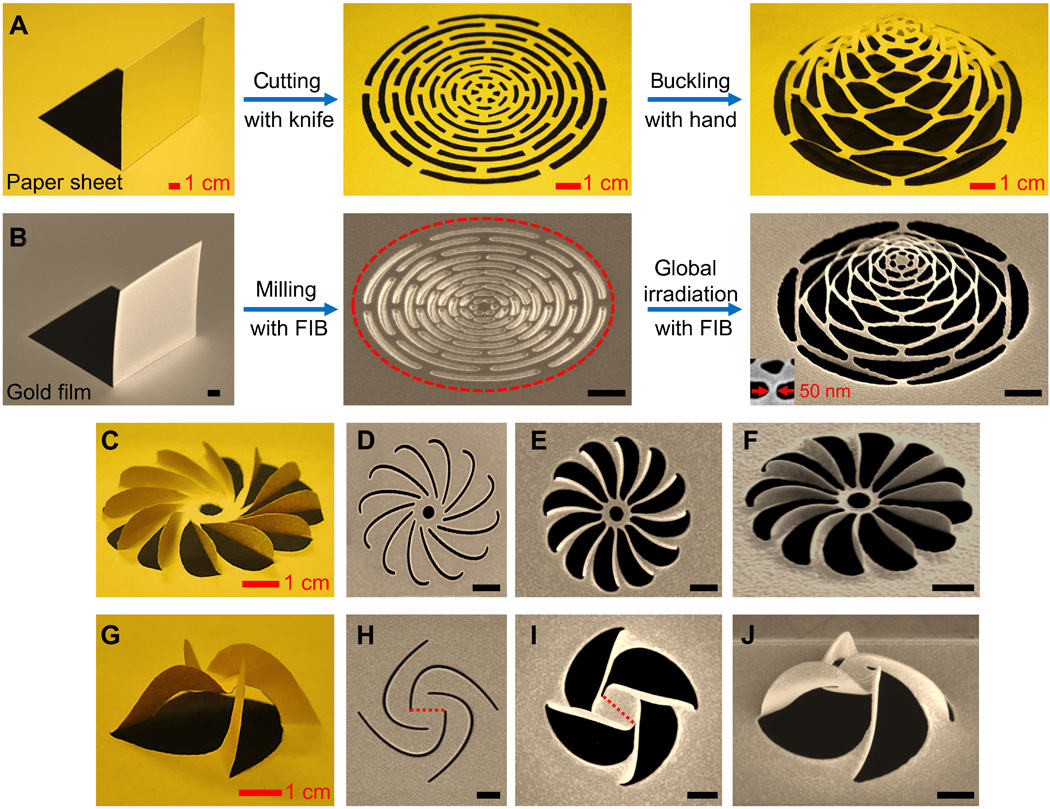
\includegraphics[width=0.6\linewidth]{figures/kirigami_example.jpeg}
		\caption{Example of transistion from macro- to nano-kirigami using a focused ion-beam (FIB) (Nano-kirigami with giant optical chirality, ZHIGUANG LIU, 2018).}
	\end{figure}	

\end{frame}

\begin{frame}
	\frametitle{Master's thesis}
	\framesubtitle{Choosing a cut pattern}
	\begin{itemize}
		\item Kirigami design on macroscale.
	\end{itemize}
	\begin{figure}
		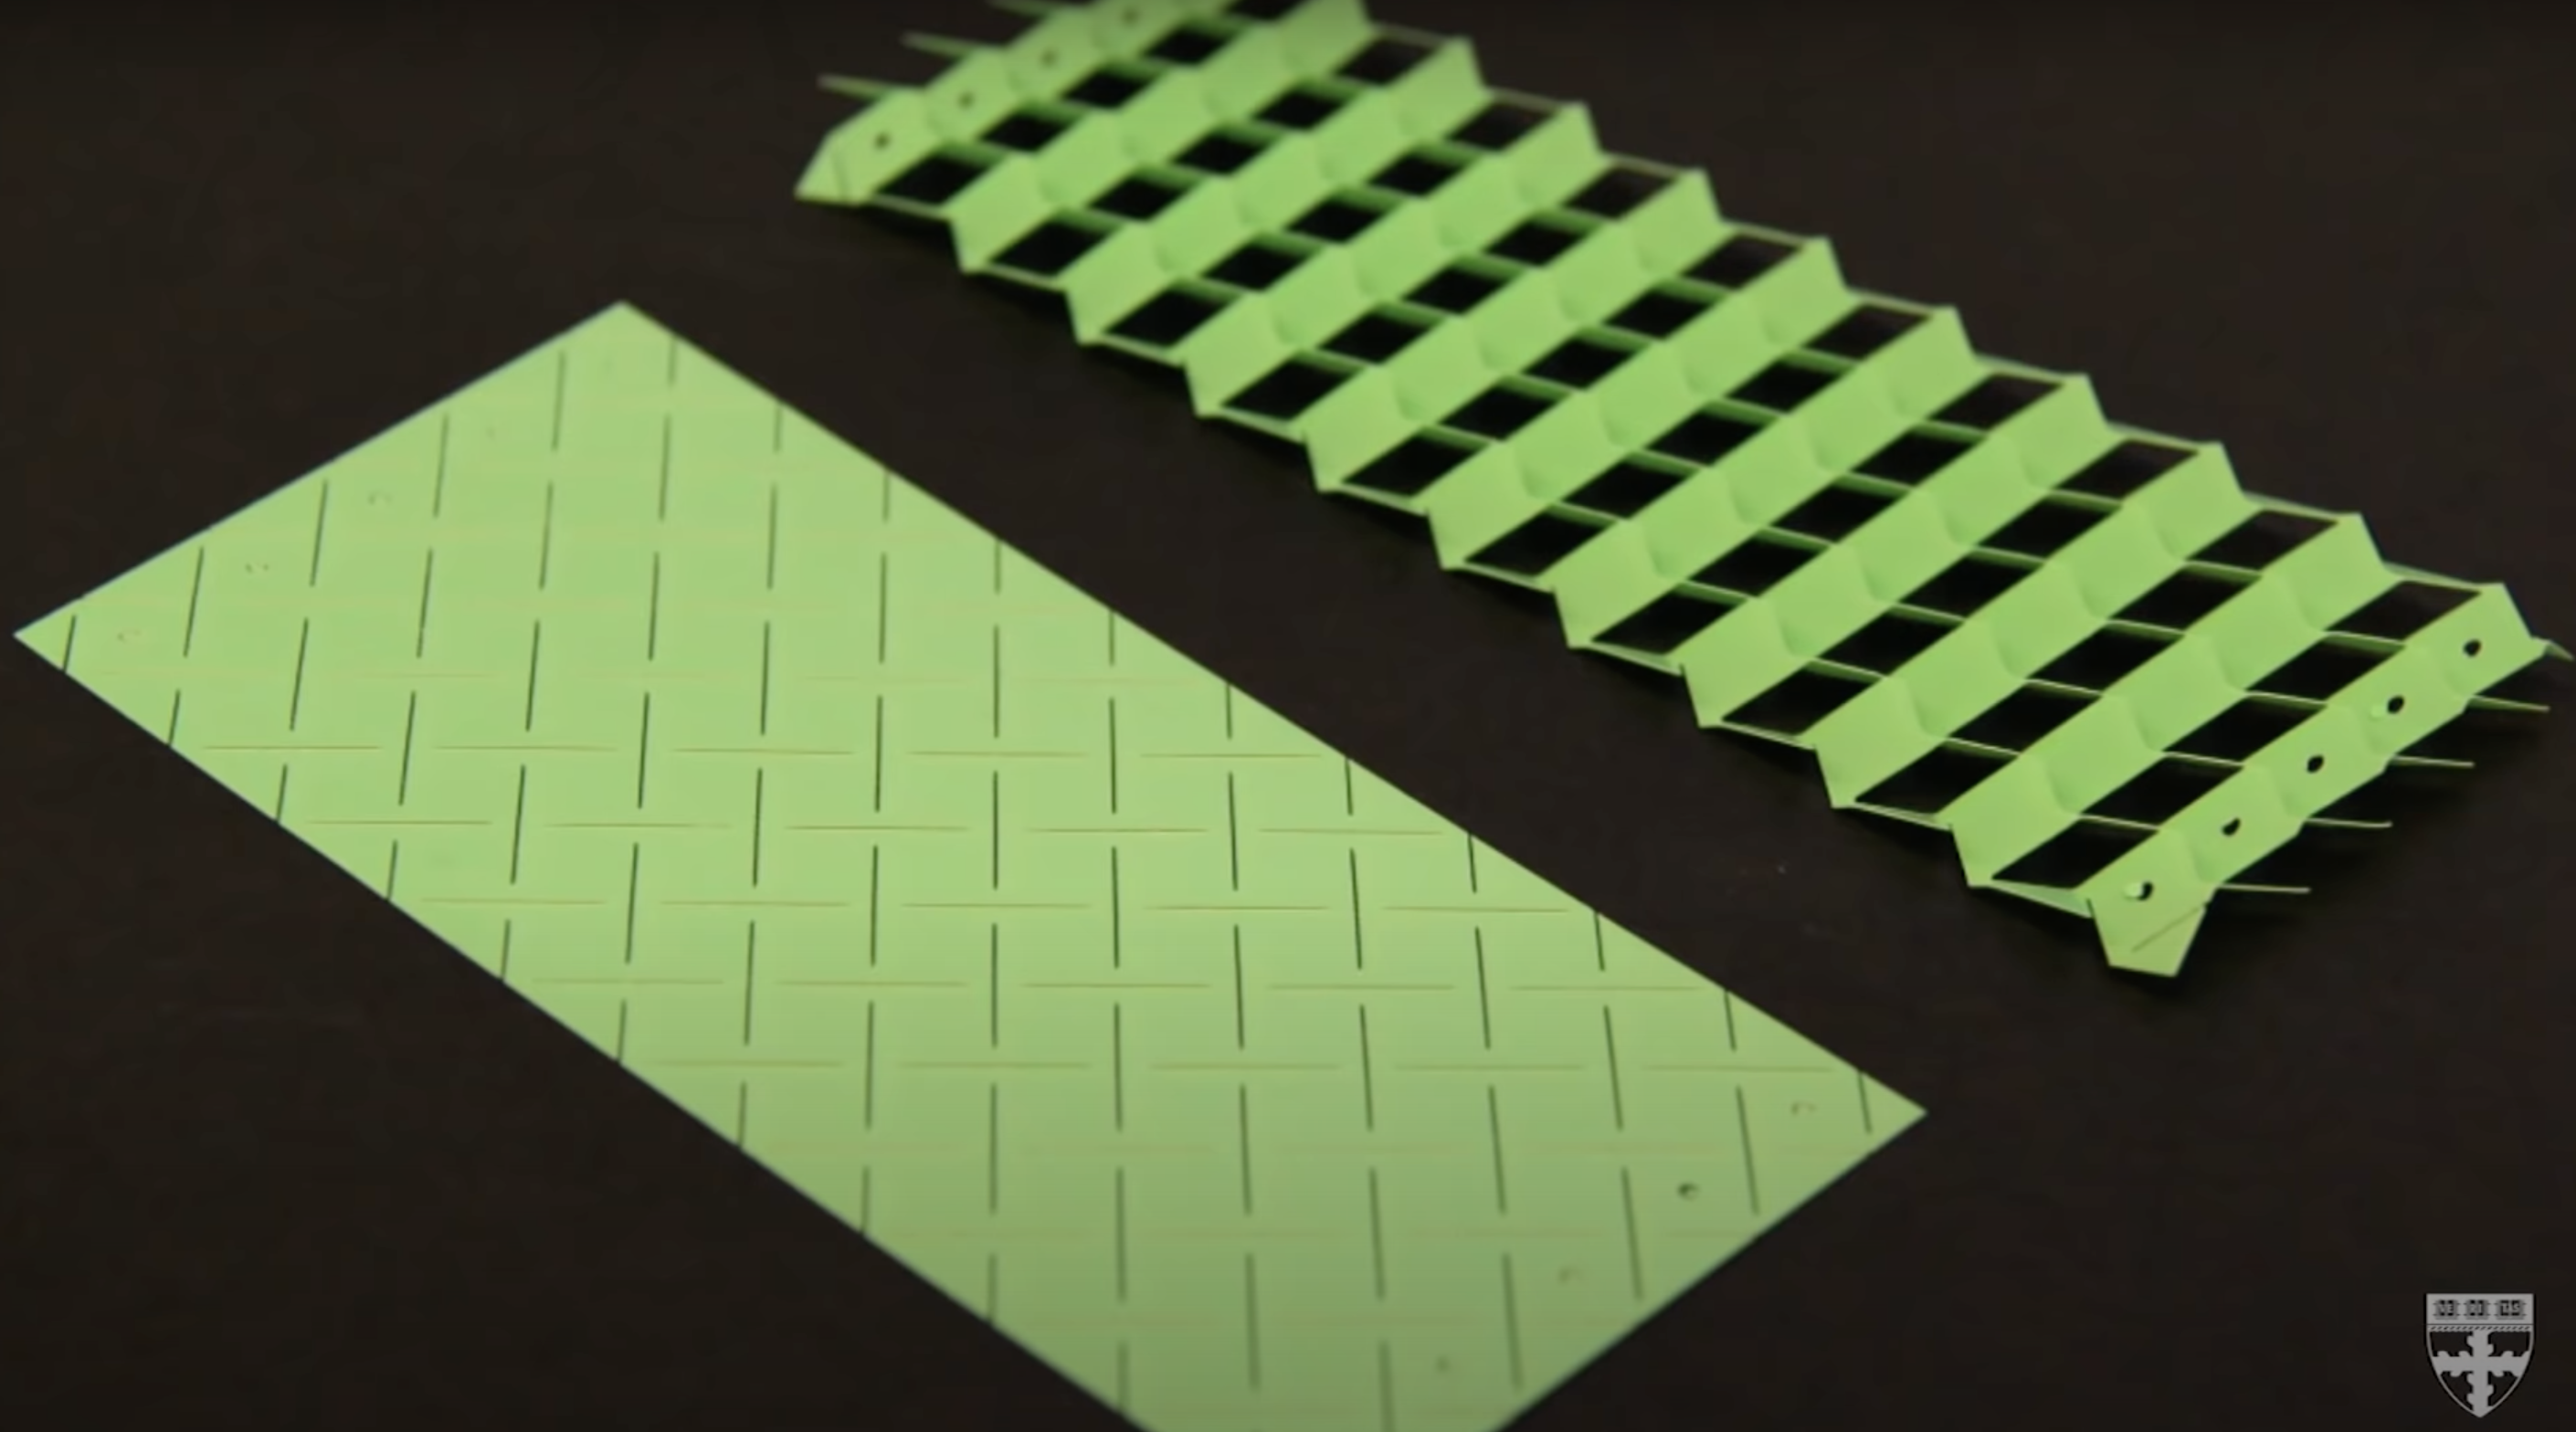
\includegraphics[width=0.6\linewidth]{figures/kirigami_pattern_inspiration.png}
		\caption{New pop-up strategy inspired by cuts, not folds - Leah Burrows, Harvard John A. Paulson School of Engineering and Applied Sciences.}
	\end{figure}	
\end{frame}



\begin{frame}
	\frametitle{Master's thesis}
	\framesubtitle{Translating patterns to MD}
	\begin{figure}
		\centering    
		\movie[open]{
\includegraphics[width=\textheight, keepaspectratio]{figures/vacuum_stretch.png}}{figures/vacuum_stretch.mov}
		\caption{Kirigami sheet stretch in vaccuum.}
   \end{figure} 
\end{frame}


\begin{frame}
	\frametitle{Master's thesis}
	\framesubtitle{Investigating 3D buckling}
	\begin{figure}
		\centering    
		\movie[open]{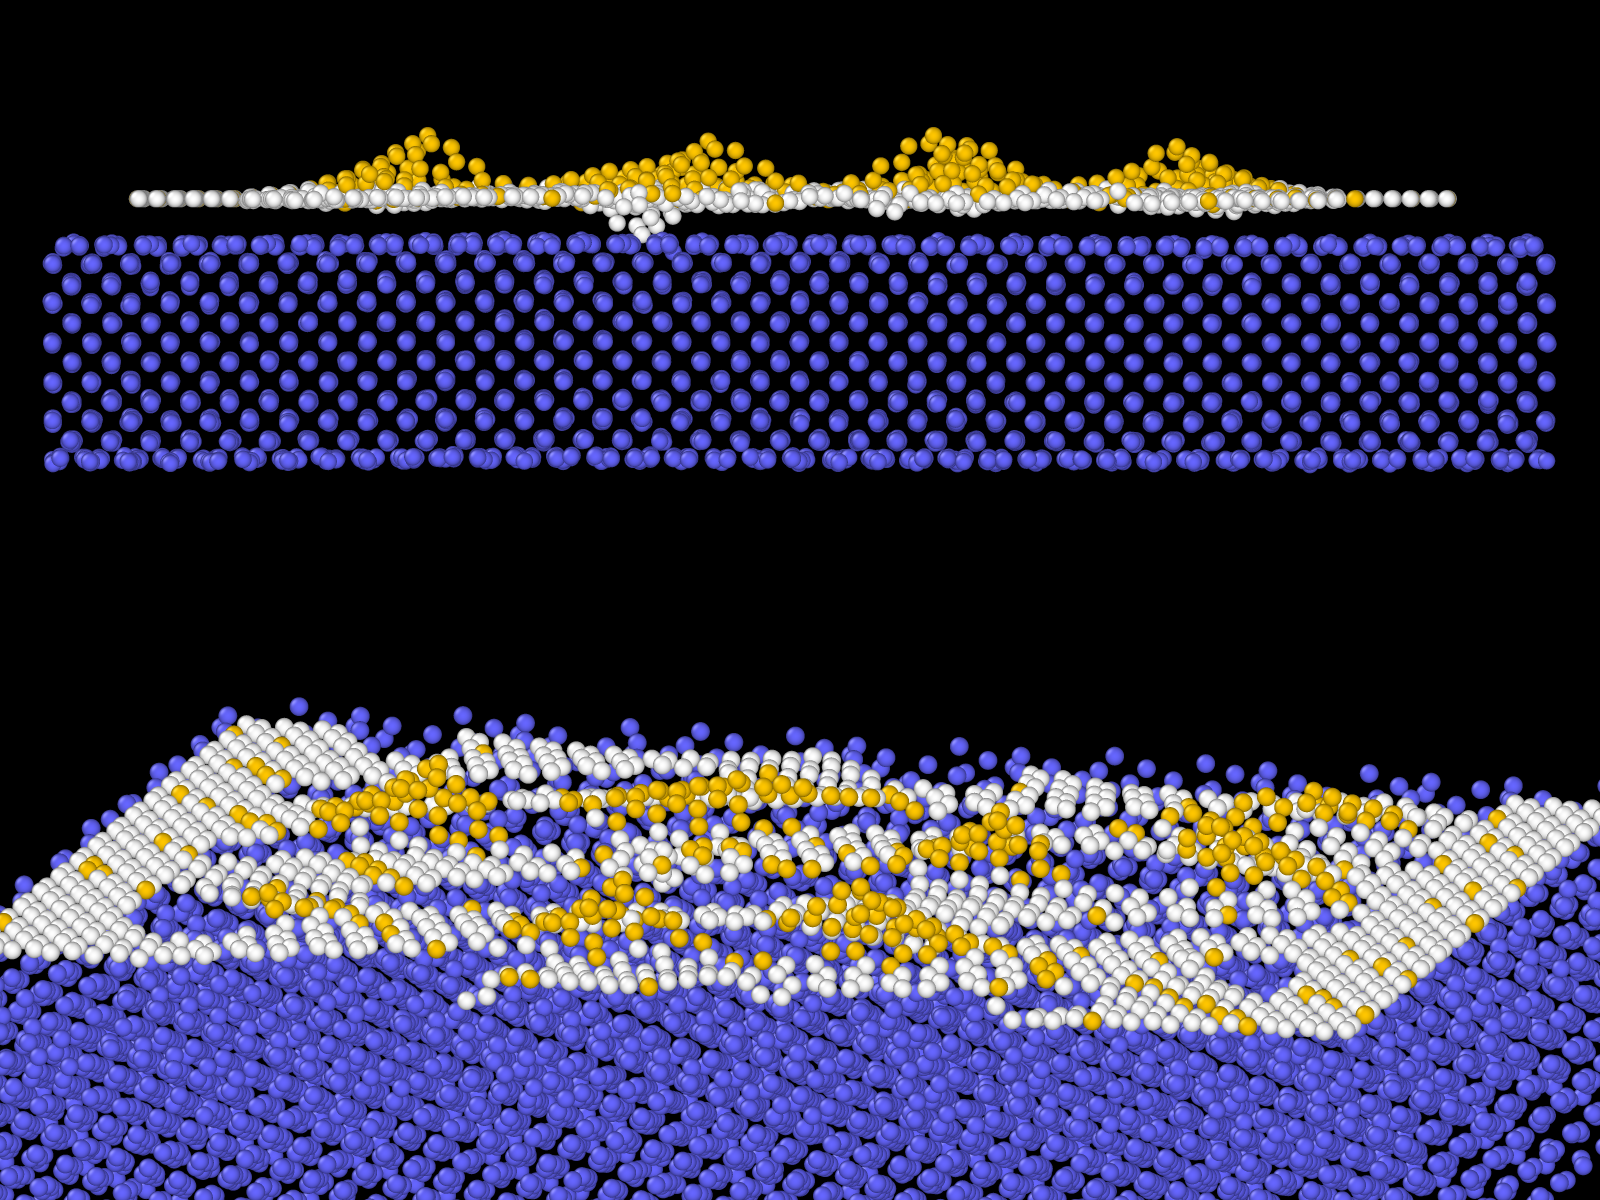
\includegraphics[width=0.95\textheight, keepaspectratio]{figures/contact_stretch.png}}{figures/contact_stretch.mov}
		\caption{Kirigami stretch in contact with Si-substrate.}
	\end{figure} 
\end{frame}


\begin{frame}
	\frametitle{Master's thesis}
	\framesubtitle{Investigating 3D buckling}
	\begin{figure}
		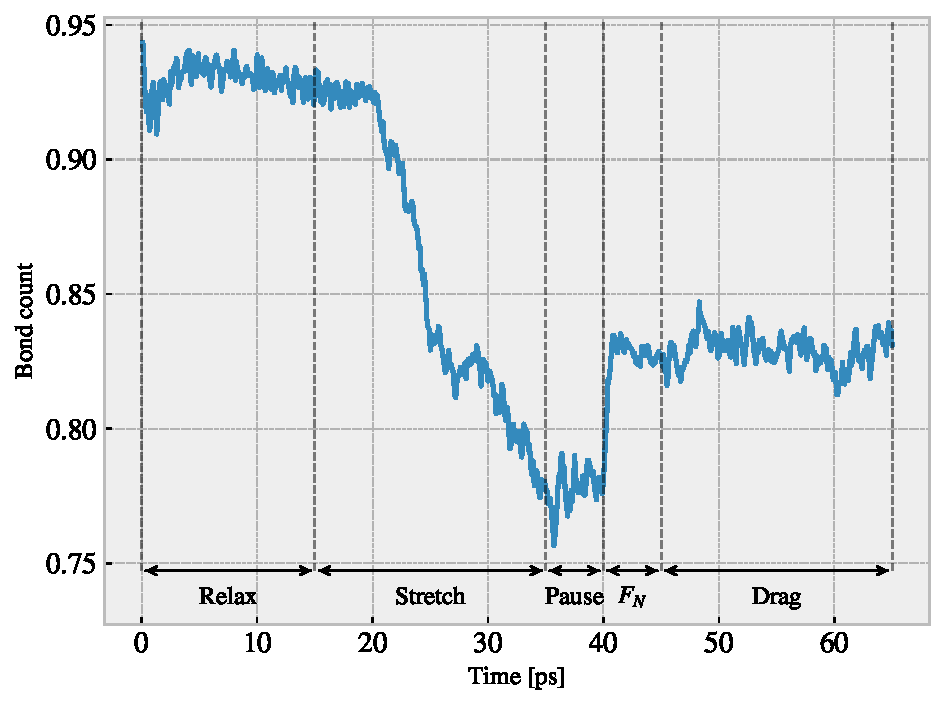
\includegraphics[width=0.7\linewidth]{figures/contact_pct.pdf}
		\caption{Contact area approximation: Number of C-Si bonds within a threshold distance of 110\% the LJ interaction equilibrium distance.}
	\end{figure}	
\end{frame}


\begin{frame}
	\frametitle{Master's thesis}
	\framesubtitle{Friction stretch dependency}
	\begin{figure}
		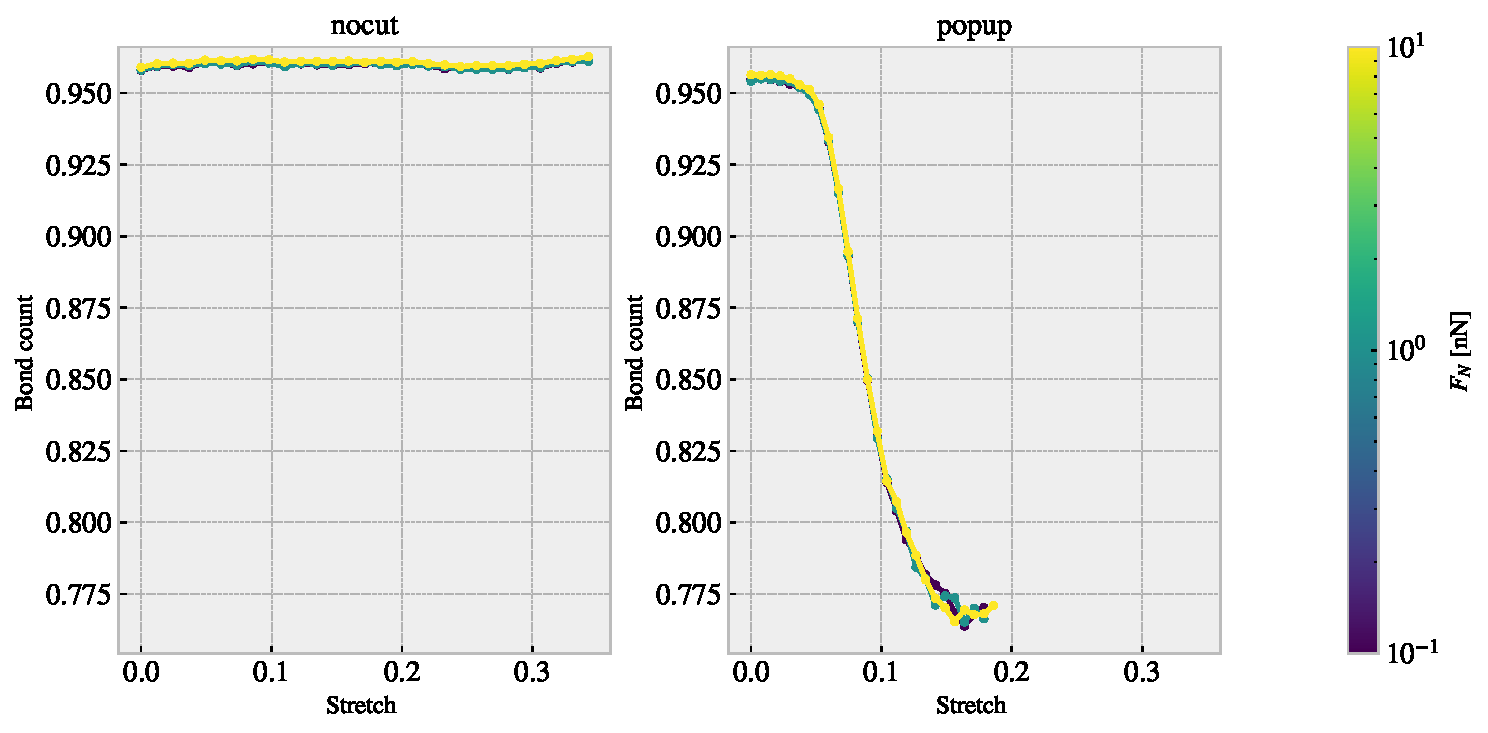
\includegraphics[width=\linewidth]{figures/multi_3.pdf}
		\caption{Relative number of bonds between sheet and substrate as a function of stretch of the sheet with and without cuts.}
	\end{figure}	
\end{frame}

\begin{frame}
	\frametitle{Master's thesis}
	\framesubtitle{Friction stretch dependency}
	\begin{figure}
		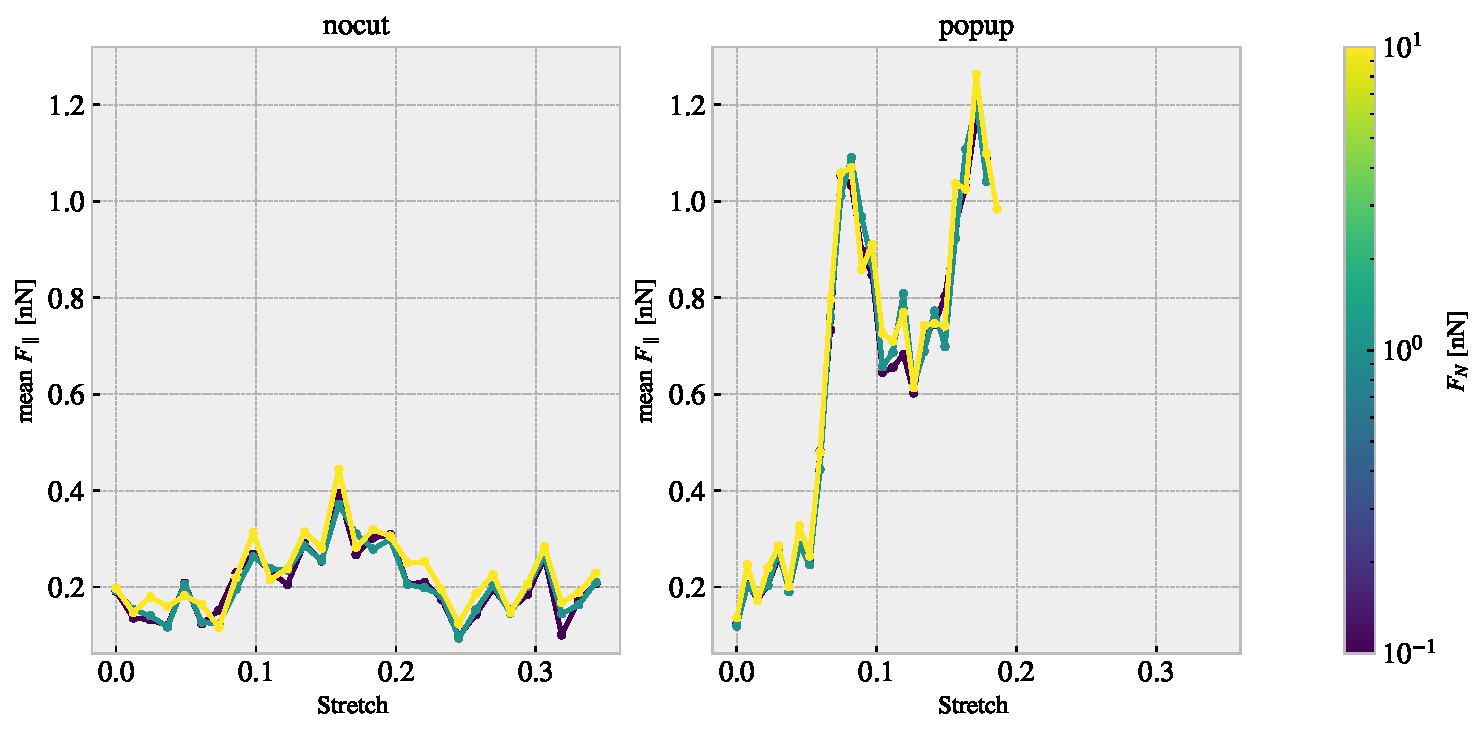
\includegraphics[width=\linewidth]{figures/multi_2.pdf}
		\caption{Mean friction force $F_{\parallel}$ parallel to drag direction as a function of stretch of the sheet with and without cuts.}
	\end{figure}	
\end{frame}


\begin{frame}
	\frametitle{Master's thesis}
	\framesubtitle{Friction stretch dependency}
	\begin{figure}
		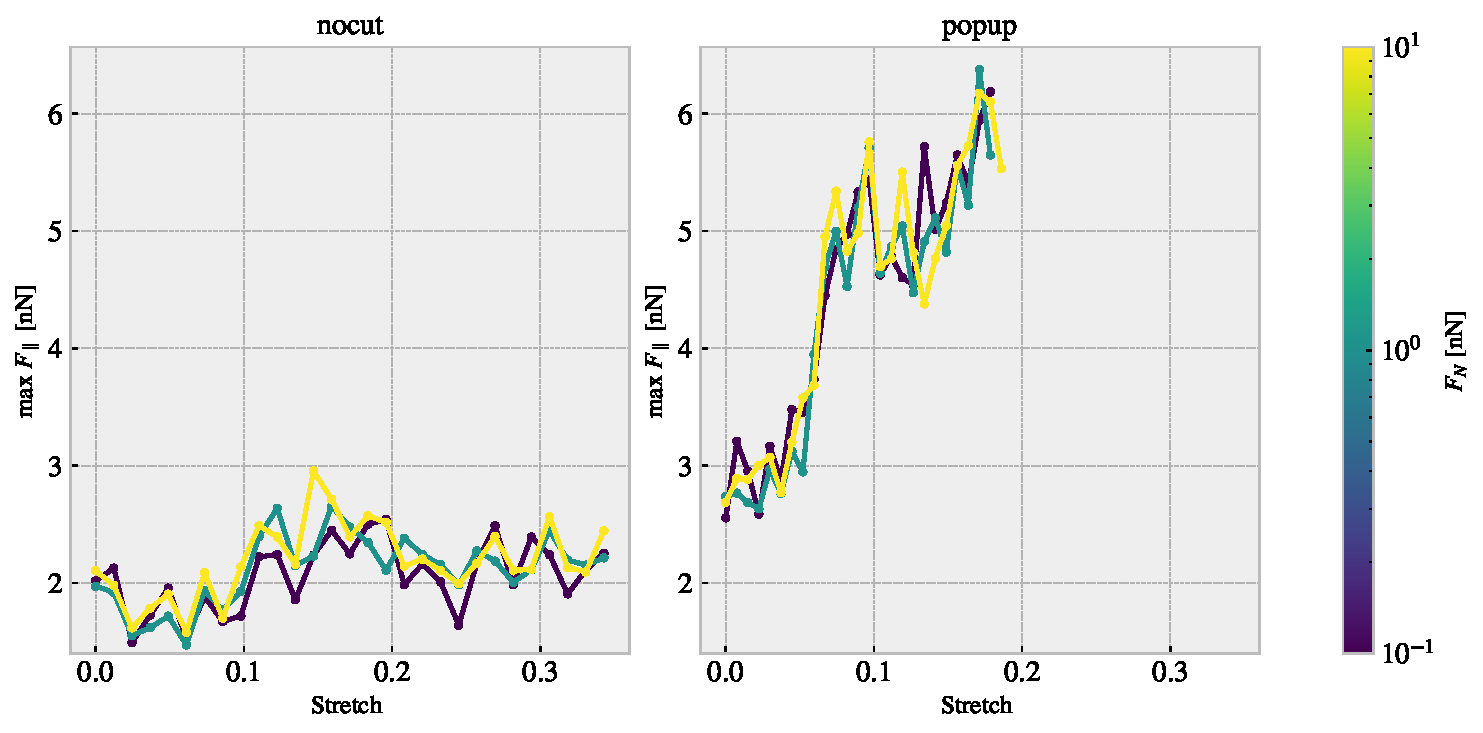
\includegraphics[width=\linewidth]{figures/multi_1.pdf}
		\caption{Max friction force $F_{\parallel}$ parallel to drag direction as a function of stretch of the sheet with and without cuts.}
	\end{figure}	
\end{frame}




\begin{frame}
	\frametitle{Master's thesis}
	\framesubtitle{Inverse design}
	\textit{Designing complex architectured materials with generative adversarial networks, YUNWEI MAO, 2020.}
	\begin{figure}
		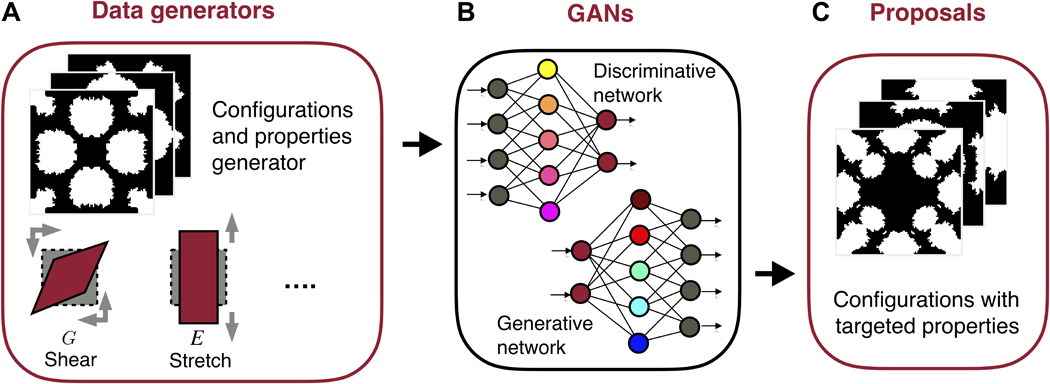
\includegraphics[width=0.8\linewidth]{figures/ML_procedure.jpeg}
		\caption{(A) Data generators to generate datasets of configurations and properties of architectured materials. (B) GANs trained by the datasets. (C) New designs of architectured materials with the targeted properties proposed by the GANs.}
	\end{figure}
\end{frame}

\begin{frame}
	\frametitle{Master's thesis}
	\framesubtitle{Possible application: Nanomachine for negative friction coefficient}

	\begin{align*}
		\left.\begin{aligned}
			\text{Normal force} &: F_f = k \cdot F_N \\
			\text{Stretch} &: F_f \sim s \cdot \text{stretch}  \\
			\text{Nanomachine}&: \text{stretch} = \pm R \cdot F_n
		  \end{aligned}\right\} \Longrightarrow F_f \propto \underbrace{(k \pm sR)}_{\mu} \cdot F_n
	\end{align*}
	
	% \begin{align*}
	% 	\left.\begin{aligned}
	% 		\text{Contact area} &: A_0 = k \cdot F_N \\
	% 		\text{Kirigami} &: A = A_0 - s_1 \cdot \text{stretch} \\
	% 		\text{Nanomachine}&: \text{stretch} = s_2 \cdot F_n
	% 	  \end{aligned}\right\} \Longrightarrow F_f \propto A = \underbrace{(k - s_1 \cdot s_2)}_{\mu} \cdot F_N
	% \end{align*}
	
	\begin{figure}
		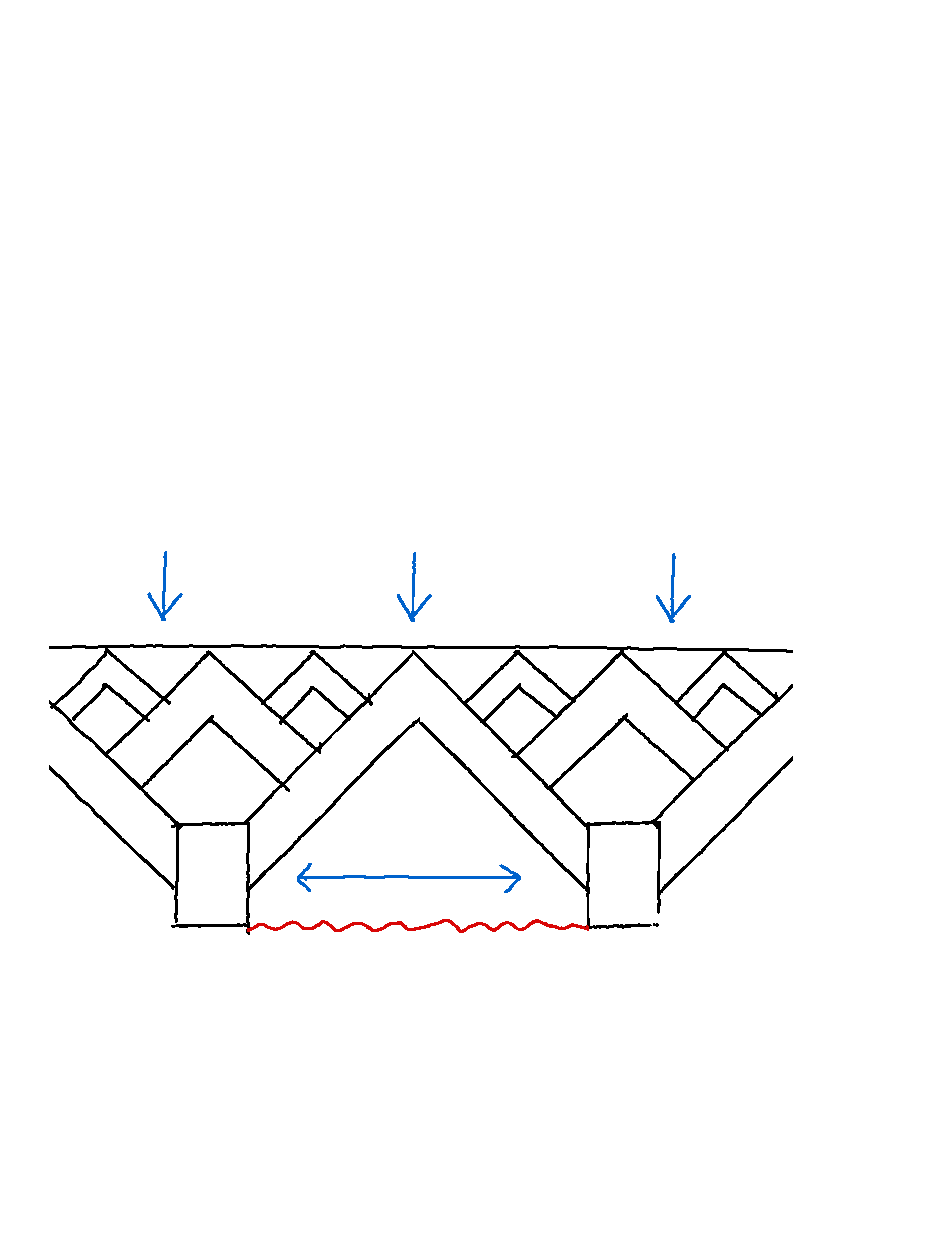
\includegraphics[width=0.6\linewidth]{figures/nanomachine.pdf}
		\caption{Sketch for nanomachine coupling normal force and stretch. Black represents nanomachine components and red the sheet.}
	\end{figure}	
	
\end{frame}



	



\end{document} 


